\documentclass[journal]{IEEEtran}

\usepackage[T1]{fontenc}
\usepackage{cite}
\usepackage{amsmath,amssymb,amsfonts}
\usepackage{algorithmic}
\usepackage{graphicx}
\usepackage{textcomp}
\usepackage{xcolor}
\usepackage{booktabs}
\usepackage{multirow}
\usepackage{array}
\usepackage{tikz}
\usepackage{pgfplots}
\usepackage{url}
\usetikzlibrary{arrows.meta,positioning,fit,calc,shapes.geometric}
\pgfplotsset{compat=1.18}

\newcommand{\modelname}{A$^2$SNN}
\newcommand{\argmax}{\mathop{\mathrm{arg\,max}}}

\begin{document}

\title{A Hardware-Aware Lightweight Spiking Neural Network with Adaptive Event-Driven Inference for Resource-Constrained Microcontrollers}

\author{Author Name,
        Department Name,
        University Name%
\thanks{Manuscript prepared as an Overleaf-ready journal draft. Replace author, affiliation, funding, and experimental values after hardware measurement.}}

\markboth{Journal Draft, 2026}%
{Author \MakeLowercase{\textit{et al.}}: Hardware-Aware Lightweight Spiking Neural Network}

\maketitle

\begin{abstract}
Spiking neural networks (SNNs) are attractive for edge intelligence because their event-driven computation can reduce unnecessary arithmetic when input activity is sparse. However, many efficient SNN demonstrations are designed around FPGA or neuromorphic substrates, where parallel logic, local buffering, and custom datapaths can be assumed. Commodity microcontrollers expose a different bottleneck profile: limited SRAM, flash bandwidth, sequential instruction execution, interrupt overhead, and tight energy budgets. This paper presents \modelname, an adaptive asynchronous SNN co-design for microcontroller-class inference. The proposed design jointly optimizes spike generation, quantized leaky-integrate-and-fire dynamics, sparse event scheduling, and confidence-aware early termination. The model uses 1-bit spike events, INT8 synaptic weights, integer membrane states, and shift-based leakage to avoid floating-point operations during inference. A corresponding microcontroller execution architecture is specified with flash-resident weights, SRAM-resident states, an event scheduler, sparse synaptic update loops, and an early-exit readout. The study is framed as a reproducible journal-style methodology with accuracy, latency, memory, cycle, power, and energy metrics. The intended contribution is not a direct port of an FPGA accelerator, but a hardware-aware SNN formulation whose algorithmic sparsity and inference duration adapt to microcontroller constraints.
\end{abstract}

\begin{IEEEkeywords}
Spiking neural network, microcontroller, TinyML, neuromorphic computing, event-driven inference, quantization, early exit, embedded machine learning.
\end{IEEEkeywords}

\section{Introduction}
Edge machine learning increasingly requires inference under severe memory, latency, and energy constraints. Microcontrollers are especially important in this setting because they are inexpensive, widely deployed, and suitable for battery-powered sensing platforms. Yet their computational model remains fundamentally sequential: even when vector extensions or small accelerators are available, the memory hierarchy, instruction budget, and real-time scheduling constraints differ substantially from FPGA and GPU platforms.

Spiking neural networks offer a promising direction because computation is triggered by discrete events rather than dense activations \cite{roy2019towards,pfeiffer2018deep}. In principle, an inactive input should not require a full multiply-accumulate pass through every neuron. In practice, this advantage is only realized when the model, numerical representation, memory layout, and inference scheduler are designed together. A dense SNN implemented as a conventional layer loop may preserve the biological terminology of spikes while losing the computational benefit that made the model attractive.

Existing FPGA-oriented SNN accelerators exploit specialized programmable logic and parallel hardware resources. Their architectures commonly use time-multiplexed spike delivery, pipelined neuron updates, and local datapaths to achieve efficient inference. A direct deployment of such designs on a commodity microcontroller does not address the tighter SRAM, flash-access, sequential-compute, and energy constraints of MCU execution. This paper therefore investigates a hardware-aware SNN co-design in which spike generation, integer LIF dynamics, sparse event scheduling, and inference duration are jointly optimized for MCU deployment.

The proposed model, called \modelname{} for Adaptive Asynchronous Spiking Neural Network, is designed around four principles:
\begin{itemize}
    \item adaptive spike encoding reduces activity for low-information inputs;
    \item multiplier-free LIF dynamics use integer states, INT8 weights, and shift-based leakage;
    \item sparse event scheduling updates only neurons connected to active spikes;
    \item confidence-aware early exit stops inference when the output margin is sufficient.
\end{itemize}

The central claim is methodological: for MCU-class inference, the SNN architecture should be shaped by the platform's actual bottlenecks rather than copied from a hardware substrate with different assumptions.

\section{Related Work}
\subsection{Spiking Neural Networks}
SNNs encode information using discrete spike events and temporal state dynamics. Compared with conventional artificial neural networks (ANNs), SNNs can exploit temporal sparsity because neurons communicate only when spikes occur. Leaky-integrate-and-fire neurons are widely used because they provide a simple state update rule with a thresholding mechanism suitable for digital implementation. Modern SNN training commonly uses surrogate-gradient methods to optimize nondifferentiable spike functions \cite{neftci2019surrogate,zenke2018superspike}.

\subsection{Hardware-Aware Neural Inference}
Hardware-aware neural network design has become a core theme in TinyML and edge AI \cite{banbury2021benchmarking}. Quantization, pruning, memory-aware scheduling, and operator fusion are commonly used to reduce inference cost \cite{jacob2018quantization,han2016eie}. For microcontrollers, however, model size alone is not sufficient: flash access patterns, peak SRAM, interrupt timing, and control-flow overhead strongly influence real deployment performance.

\subsection{SNN Accelerators}
FPGA and neuromorphic SNN accelerators can use custom datapaths, parallel neuron blocks, and local memories. Neuromorphic chips such as TrueNorth and Loihi demonstrate the potential efficiency of event-driven computation in specialized substrates \cite{merolla2014truenorth,davies2018loihi}, but their design choices do not automatically translate to low-cost microcontrollers. \modelname{} is positioned as an MCU-oriented co-design rather than an FPGA microarchitecture replica.

\section{Problem Formulation}
Let $x \in \mathbb{R}^{d}$ denote an input sample and let $T_{\max}$ denote the maximum number of inference timesteps. A conventional fixed-duration SNN evaluates all samples for $T_{\max}$ timesteps and accumulates output spikes or membrane states before classification. This can waste computation on samples that become separable early.

The objective is to learn and deploy an SNN inference procedure
\begin{equation}
    \hat{y} = f_{\theta}(x; T_x),
\end{equation}
where the effective inference duration $T_x \leq T_{\max}$ is input-dependent. The deployment target is a microcontroller with constrained flash, SRAM, and cycle budget. The inference engine should minimize expected cost
\begin{equation}
    \mathcal{C} = \lambda_1 \mathbb{E}[T_x] + \lambda_2 \mathbb{E}[N_{\mathrm{spk}}] + \lambda_3 M_{\mathrm{SRAM}} + \lambda_4 M_{\mathrm{Flash}},
\end{equation}
subject to an accuracy constraint
\begin{equation}
    \mathrm{Acc}(f_{\theta}) \geq \mathrm{Acc}_{\mathrm{target}}.
\end{equation}
Here $N_{\mathrm{spk}}$ is the number of processed spike events, $M_{\mathrm{SRAM}}$ is peak SRAM usage, and $M_{\mathrm{Flash}}$ is flash-resident model storage.

\section{Proposed Model Architecture}
\subsection{Overview}
\modelname{} consists of an adaptive event encoder, a quantized sparse SNN core, an integer LIF state update, and a confidence-aware readout. Fig.~\ref{fig:model_architecture} shows the model-level architecture.

\begin{figure}[t]
\centering
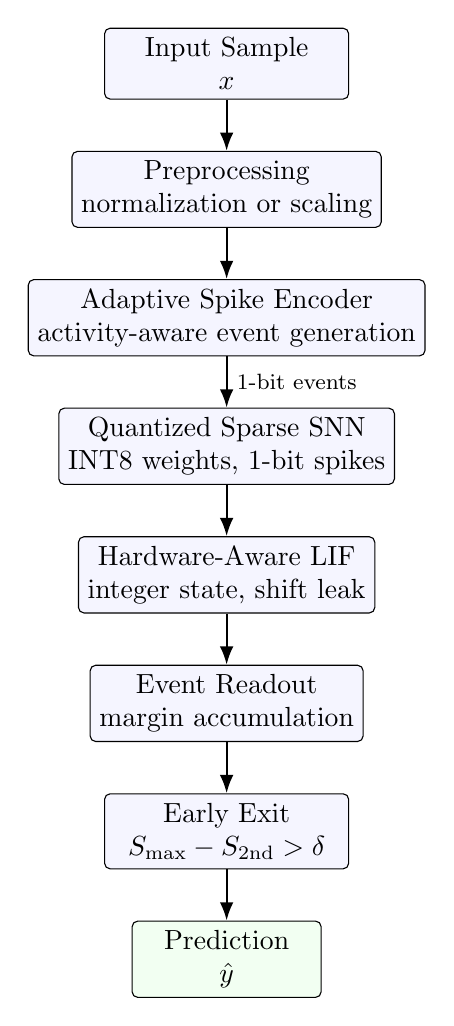
\begin{tikzpicture}[
    node distance=6.5mm,
    block/.style={draw, rounded corners=2pt, align=center, minimum width=31mm, minimum height=8mm, fill=blue!4},
    small/.style={draw, rounded corners=2pt, align=center, minimum width=24mm, minimum height=7mm, fill=green!5},
    arrow/.style={-Latex, thick}
]
\node[block] (input) {Input Sample\\$x$};
\node[block, below=of input] (pre) {Preprocessing\\normalization or scaling};
\node[block, below=of pre] (enc) {Adaptive Spike Encoder\\activity-aware event generation};
\node[block, below=of enc] (snn) {Quantized Sparse SNN\\INT8 weights, 1-bit spikes};
\node[block, below=of snn] (lif) {Hardware-Aware LIF\\integer state, shift leak};
\node[block, below=of lif] (read) {Event Readout\\margin accumulation};
\node[block, below=of read] (exit) {Early Exit\\$S_{\max}-S_{\mathrm{2nd}}>\delta$};
\node[small, below=of exit] (pred) {Prediction\\$\hat{y}$};
\draw[arrow] (input) -- (pre);
\draw[arrow] (pre) -- (enc);
\draw[arrow] (enc) -- node[right, font=\footnotesize]{1-bit events} (snn);
\draw[arrow] (snn) -- (lif);
\draw[arrow] (lif) -- (read);
\draw[arrow] (read) -- (exit);
\draw[arrow] (exit) -- (pred);
\end{tikzpicture}
\caption{Model architecture of \modelname. The inference path is event-driven and supports input-dependent termination.}
\label{fig:model_architecture}
\end{figure}

\subsection{Adaptive Spike Encoding}
For each input dimension $i$, the encoder maps a normalized value $x_i$ and an activity statistic $a(x)$ to a spike probability or thresholded event rule:
\begin{equation}
    r_i = \phi(x_i, a(x)).
\end{equation}
The function $\phi(\cdot)$ is selected so that low-information inputs generate fewer events while high-contrast or high-activity inputs retain sufficient temporal resolution. A simple implementation is
\begin{equation}
    z_i[t] = \mathbb{I}\left(q(x_i) + \eta_i[t] > \tau(a(x))\right),
\end{equation}
where $z_i[t] \in \{0,1\}$ is the input spike, $q(\cdot)$ is an integer quantizer, $\eta_i[t]$ is a deterministic or pseudo-random temporal dither, and $\tau(\cdot)$ is an activity-dependent threshold.

\subsection{Quantized LIF Dynamics}
The membrane update for neuron $j$ is implemented without multiplication in the leakage path:
\begin{equation}
    V_j[t+1] = V_j[t] - (V_j[t] \gg k) + I_j[t] - \Theta s_j[t],
\end{equation}
where $V_j$ is an INT16 or INT32 membrane state, $k$ is the leak-shift parameter, $\Theta$ is an integer threshold, and $s_j[t]$ is the output spike. The synaptic current is accumulated from active presynaptic spikes:
\begin{equation}
    I_j[t] = \sum_{i \in \mathcal{A}_t} w_{ij},
\end{equation}
where $\mathcal{A}_t = \{i \mid z_i[t]=1\}$ and $w_{ij}$ is an INT8 weight.

\subsection{Sparse Event Scheduling}
Instead of evaluating all neurons at each timestep, the MCU scheduler iterates through active events:
\begin{algorithmic}[1]
\STATE Initialize membrane states and output counters.
\FOR{$t=1$ to $T_{\max}$}
    \STATE Generate active input spikes $\mathcal{A}_t$.
    \FOR{each active spike $i \in \mathcal{A}_t$}
        \STATE Read compressed outgoing weight list for spike $i$.
        \STATE Accumulate only connected postsynaptic states.
    \ENDFOR
    \STATE Apply integer leak and threshold to touched neurons.
    \STATE Update class counters and output margin.
    \IF{$S_{\max} - S_{\mathrm{2nd}} > \delta(t)$}
        \STATE Stop and return $\hat{y}=\argmax_c S_c$.
    \ENDIF
\ENDFOR
\STATE Return $\hat{y}=\argmax_c S_c$.
\end{algorithmic}

\subsection{Confidence-Aware Early Exit}
Let $S_c[t]$ be the accumulated score for class $c$ at timestep $t$. The model exits early when
\begin{equation}
    \max_c S_c[t] - \max_{c' \neq c^*} S_{c'}[t] > \delta(t),
\end{equation}
where $c^*=\argmax_c S_c[t]$. The threshold $\delta(t)$ can be fixed, scheduled, or calibrated on a validation set. This creates an explicit accuracy-latency-energy trade-off: small $\delta$ reduces average timesteps but may harm accuracy, while large $\delta$ approaches fixed-duration inference.

\section{Microcontroller Hardware Architecture}
\subsection{Execution Substrate}
The proposed deployment assumes a commodity MCU such as an ARM Cortex-M class device or ESP32-S3 class device. The design does not require a custom FPGA fabric. Weights are stored in flash as INT8 arrays or compressed sparse rows, while membrane states, spike queues, and output counters are stored in SRAM.

\begin{figure*}[t]
\centering
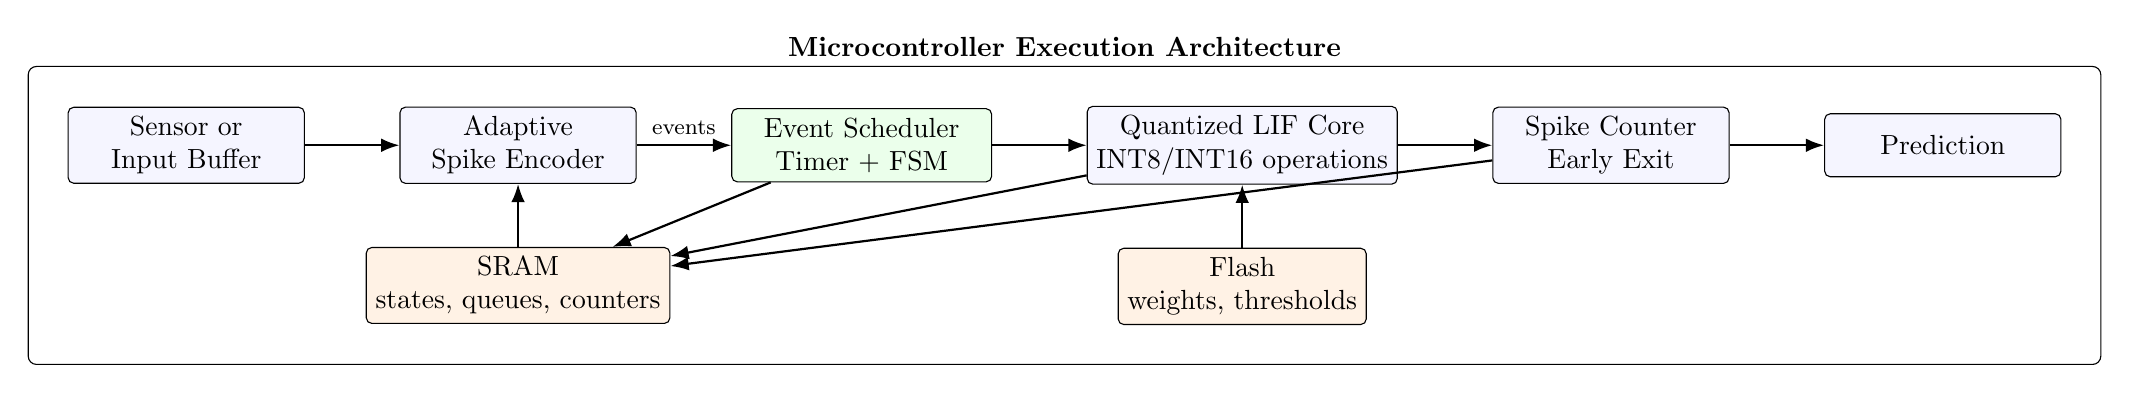
\begin{tikzpicture}[
    block/.style={draw, rounded corners=2pt, align=center, minimum width=30mm, minimum height=8mm, fill=blue!4},
    mem/.style={draw, rounded corners=2pt, align=center, minimum width=26mm, minimum height=8mm, fill=orange!10},
    ctrl/.style={draw, rounded corners=2pt, align=center, minimum width=33mm, minimum height=8mm, fill=green!8},
    arrow/.style={-Latex, thick},
    node distance=8mm and 12mm
]
\node[block] (sensor) {Sensor or\\Input Buffer};
\node[block, right=of sensor] (encoder) {Adaptive\\Spike Encoder};
\node[ctrl, right=of encoder] (sched) {Event Scheduler\\Timer + FSM};
\node[block, right=of sched] (lif) {Quantized LIF Core\\INT8/INT16 operations};
\node[mem, below=of encoder] (sram) {SRAM\\states, queues, counters};
\node[mem, below=of lif] (flash) {Flash\\weights, thresholds};
\node[block, right=of lif] (readout) {Spike Counter\\Early Exit};
\node[block, right=of readout] (pred) {Prediction};
\node[draw, rounded corners=3pt, fit=(sensor)(encoder)(sched)(lif)(sram)(flash)(readout)(pred), inner sep=5mm, label={[font=\bfseries]above:Microcontroller Execution Architecture}] (mcu) {};

\draw[arrow] (sensor) -- (encoder);
\draw[arrow] (encoder) -- node[above, font=\footnotesize]{events} (sched);
\draw[arrow] (sched) -- (lif);
\draw[arrow] (lif) -- (readout);
\draw[arrow] (readout) -- (pred);
\draw[arrow] (sram) -- (encoder);
\draw[arrow] (sched) -- (sram);
\draw[arrow] (lif) -- (sram);
\draw[arrow] (flash) -- (lif);
\draw[arrow] (readout) -- (sram);
\end{tikzpicture}
\caption{Hardware architecture for MCU deployment. The architecture emphasizes memory placement, sparse event scheduling, integer LIF updates, and early-exit readout rather than FPGA-style spatial parallelism.}
\label{fig:hardware_architecture}
\end{figure*}

\subsection{Memory Layout}
The model is partitioned into flash-resident and SRAM-resident data. Flash stores INT8 weights, layer metadata, neuron thresholds, leak parameters, and sparse index tables. SRAM stores current membrane states, active spike queues, touched-neuron flags, and class counters. This separation is critical because SRAM is usually the limiting resource for MCU inference.

\begin{table}[t]
\centering
\caption{Deployment data representation}
\label{tab:data_representation}
\begin{tabular}{lll}
\toprule
Component & Representation & Storage \\
\midrule
Input spike & 1 bit event & SRAM queue \\
Weight & INT8 & Flash \\
Membrane state & INT16/INT32 & SRAM \\
Threshold & Integer & Flash or register \\
Leak & Shift parameter $k$ & Flash or register \\
Output score & INT16/INT32 counter & SRAM \\
\bottomrule
\end{tabular}
\end{table}

\subsection{Cycle and Energy Model}
For an input sample, the approximate cycle cost is
\begin{equation}
    C_{\mathrm{inf}} \approx \sum_{t=1}^{T_x} \left(C_{\mathrm{enc}} + N_{\mathrm{evt}}[t]C_{\mathrm{evt}} + N_{\mathrm{touch}}[t]C_{\mathrm{lif}} + C_{\mathrm{read}}\right).
\end{equation}
The corresponding energy can be estimated as
\begin{equation}
    E_{\mathrm{inf}} = P_{\mathrm{avg}} \cdot L_{\mathrm{inf}},
\end{equation}
where $P_{\mathrm{avg}}$ is measured board-level or chip-level average power and $L_{\mathrm{inf}}$ is inference latency.

\section{Training and Deployment Flow}
Training is performed on a workstation using surrogate gradients or ANN-to-SNN conversion followed by calibration. The deployment flow is:
\begin{enumerate}
    \item train the SNN with hardware-aware constraints;
    \item apply quantization-aware training or post-training quantization;
    \item export INT8 weights, integer thresholds, and leak parameters;
    \item pack sparse weight tables for flash access;
    \item compile MCU firmware with the event scheduler and LIF kernel;
    \item measure accuracy, latency, memory, cycles, power, and energy.
\end{enumerate}

\section{Experimental Methodology}
\subsection{Datasets}
The first evaluation can use MNIST or Fashion-MNIST for rapid validation, followed by CIFAR-10 for a more demanding vision benchmark. If the final thesis direction is continual learning, split CIFAR-10 or split CIFAR-100 can be added as a secondary study. Dataset selection should be explicitly tied to the MCU memory budget and input resolution.

\subsection{Baselines}
The proposed method should be compared against:
\begin{itemize}
    \item a compact ANN baseline;
    \item a standard fixed-duration SNN;
    \item an INT8 SNN without sparse scheduling;
    \item an INT8 SNN with sparse scheduling;
    \item an INT8 sparse SNN with adaptive early exit;
    \item the full \modelname{} system.
\end{itemize}

\subsection{Metrics}
Table~\ref{tab:metrics} lists the minimum metrics needed for a credible hardware-aware paper.

\begin{table}[t]
\centering
\caption{Required evaluation metrics}
\label{tab:metrics}
\begin{tabular}{ll}
\toprule
Metric & Unit or description \\
\midrule
Accuracy & percent \\
Model size & KB \\
Flash usage & KB \\
Peak SRAM & KB \\
Latency & ms per sample \\
Average timesteps & timesteps per sample \\
Spike count & spikes per sample \\
CPU cycles & cycles per sample \\
Average power & mW \\
Energy & mJ per inference \\
\bottomrule
\end{tabular}
\end{table}

\subsection{Ablation Plan}
The ablation study should isolate where improvement comes from. The minimum ablation sequence is:
\begin{equation}
\begin{split}
\mathrm{ANN} &\rightarrow \mathrm{SNN} \rightarrow \mathrm{INT8\ SNN} \\
&\rightarrow \mathrm{INT8+sparse} \rightarrow \mathrm{INT8+sparse+early\ exit}\\
&\rightarrow \text{\modelname}.
\end{split}
\end{equation}
This sequence prevents the paper from attributing all gains to the full system when they may come from quantization, sparsity, or early termination individually.

\section{Expected Results Format}
The final manuscript should report measured results rather than estimated claims. Table~\ref{tab:result_template} provides a journal-ready template. Placeholder values must be replaced after MCU measurement.

\begin{table*}[t]
\centering
\caption{Result table template for final hardware measurement}
\label{tab:result_template}
\begin{tabular}{lcccccc}
\toprule
Method & Accuracy (\%) & Flash (KB) & SRAM (KB) & Latency (ms) & Avg. $T$ & Energy (mJ) \\
\midrule
Compact ANN & -- & -- & -- & -- & -- & -- \\
Fixed SNN & -- & -- & -- & -- & -- & -- \\
INT8 SNN & -- & -- & -- & -- & -- & -- \\
INT8 + Sparse & -- & -- & -- & -- & -- & -- \\
INT8 + Sparse + Early Exit & -- & -- & -- & -- & -- & -- \\
\modelname{} & -- & -- & -- & -- & -- & -- \\
\bottomrule
\end{tabular}
\end{table*}

\section{Discussion}
\modelname{} differs from FPGA-centered SNN acceleration in the location of the design pressure. FPGA designs primarily manage spatial parallelism, routing, and pipeline utilization. MCU deployment primarily manages SRAM pressure, flash bandwidth, event queue overhead, and sequential cycle count. For this reason, the same high-level SNN topology can have very different efficiency depending on whether the inference loop is dense or event-driven.

The proposed approach is strongest when spike activity is sparse and early classification margins are common. It is less advantageous when inputs produce dense spike streams or when the early-exit threshold must be set high to preserve accuracy. These limitations should be reported directly, because they define where the method is useful.

\section{Conclusion}
This paper presented \modelname, a hardware-aware adaptive SNN design for resource-constrained microcontrollers. The proposed system combines adaptive spike encoding, quantized multiplier-free LIF dynamics, sparse event scheduling, and confidence-aware early exit. The architecture is intentionally MCU-oriented: weights are flash-resident, neuron states and queues are SRAM-resident, and inference work scales with observed spike activity and required confidence. The next step is to implement the firmware kernel, measure board-level latency and power, and replace the result templates with reproducible experimental data.

\section*{Acknowledgment}
Replace this paragraph with supervisor, lab, funding, and institutional acknowledgments.

\bibliographystyle{IEEEtran}
\bibliography{references}

\end{document}
